\section{Moving from sequence to atomic structure scenario}

\subsubsection*{Downloading the atomic structure}
  
  Once identified the \iii{template} that we are going to use as structural skeleton of our sequence, we import it into \scipion with the protocol \scommand{import atomic structure} (see \ffigure{fig:import_atomic_structure} (1) and Appendix \ref{app:importAtomicStructure}). Select the option for importing the atomic structure from ID (2), write the \ttt{PDB} accession code (3) and execute the protocol (4). 
  
  \begin{figure}[H]
  \centering 
  \captionsetup{width=.9\linewidth} 
  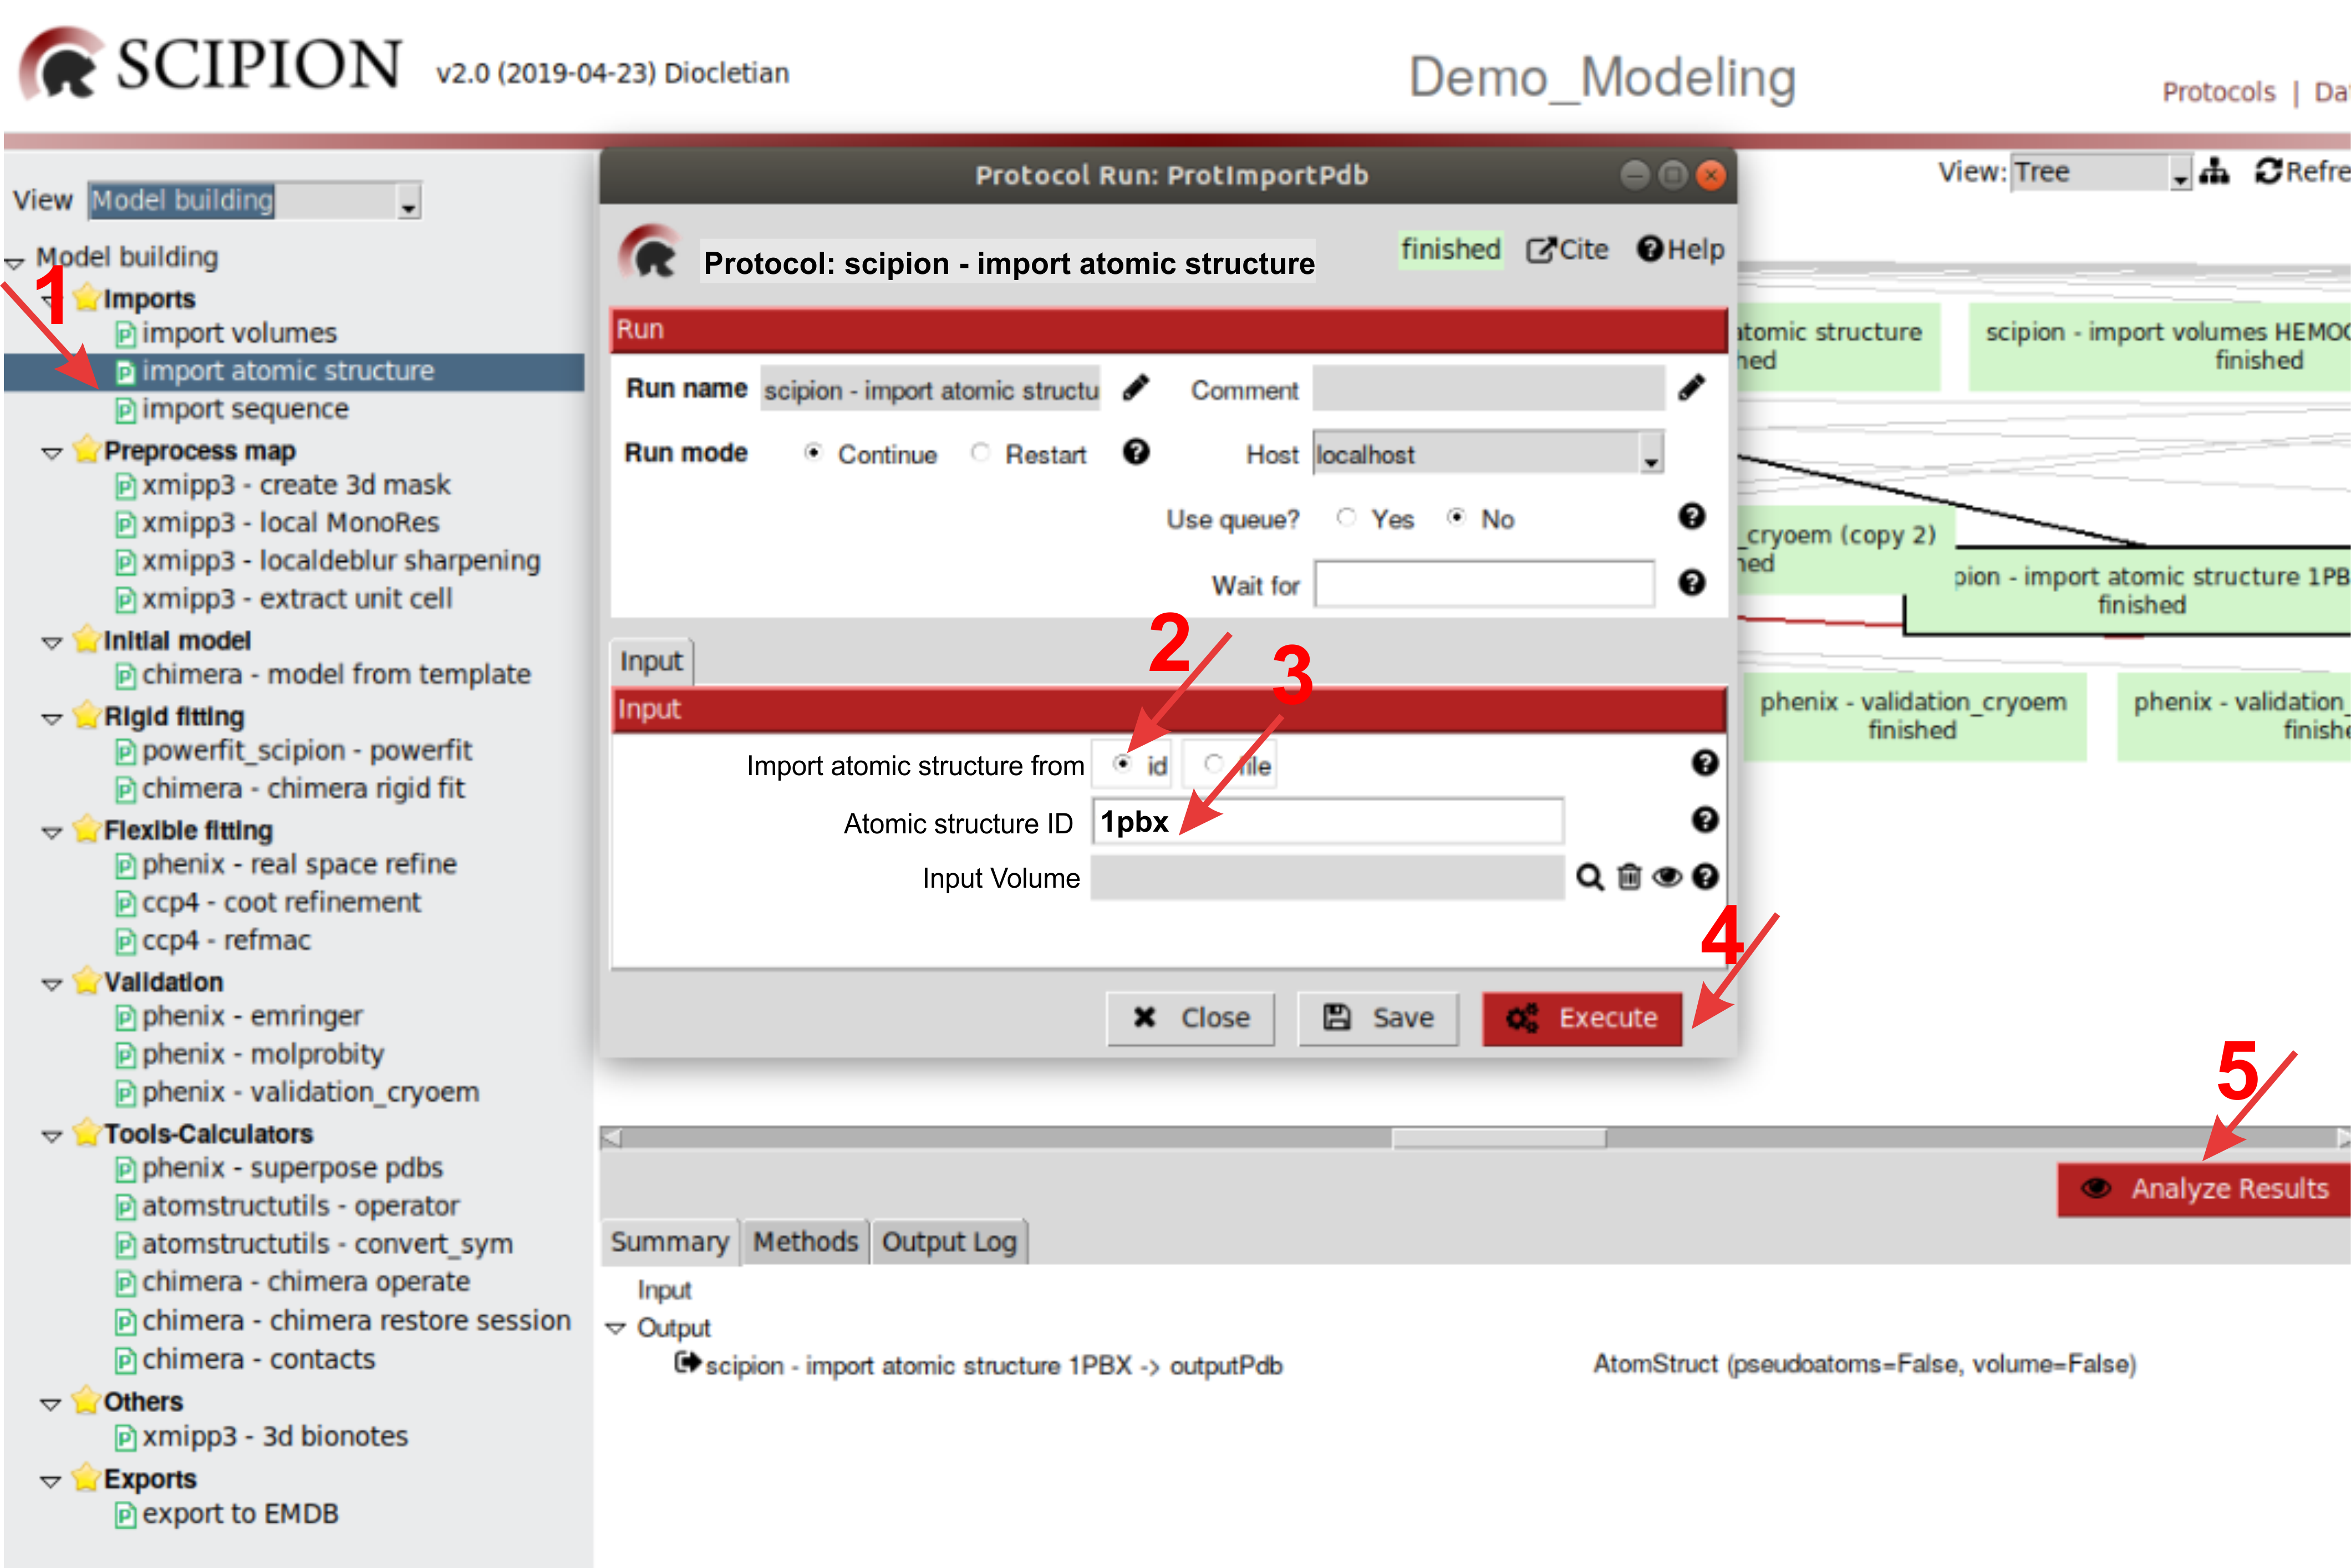
\includegraphics[width=1\textwidth]{Images/Fig10}
  \caption{Importing the atomic structure \ttt{1PBX}.}
  \label{fig:import_atomic_structure}
  \end{figure}
  You can visualize the imported structure (5) in \chimera (\ffigure{fig:chimera_visualization_structure}). By selecting chain \ttt{A} in the \chimera upper menu (1) you can distinguish the \ttt{Hgb} $\alpha$ subunit (2).
  \begin{figure}[H]
  \centering 
  \captionsetup{width=.8\linewidth} 
  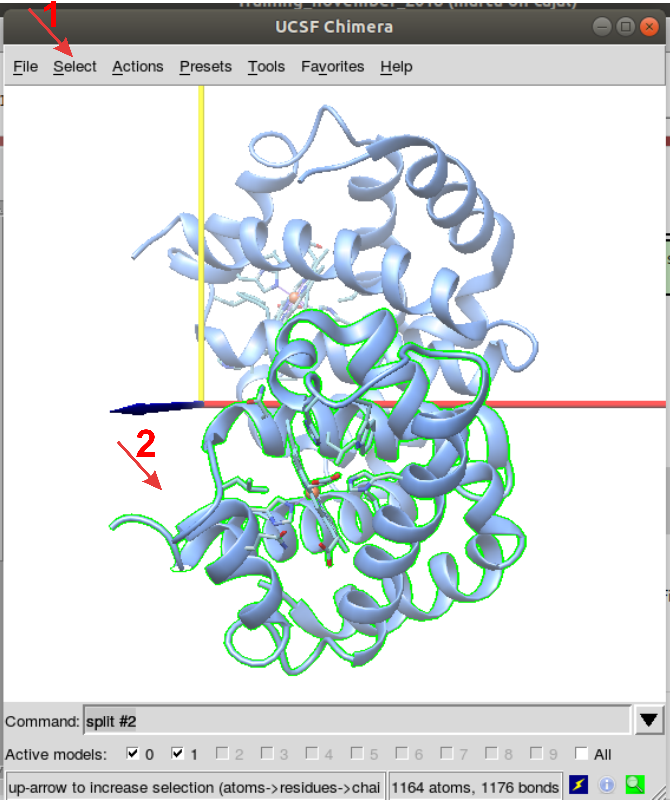
\includegraphics[width=0.80\textwidth]{Images/Fig11}
  \caption{Atomic structure \ttt{1PBX} visualized with Chimera. \ttt{Hgb} $\alpha$ subunit (chain \ttt{A}) is shown green-highlighted.}
  \label{fig:chimera_visualization_structure}
  \end{figure}
  
\subsubsection*{Structural models of human metHgb subunits from templates}

 \modeller \citep{sali1993} is one of the computational web services used by \chimera, which provides the interface to run the program. Working with \modeller requires a license key, which is provided free of charge for academic users. \modeller allows two types of modeling computations to generate theoretical models, \iii{template}-based (sequence homology) and \iii{template}-free (\iii{de novo}, only for missing segments). In this tutorial we are going to consider the first one: structure prediction by sequence homology. Requirements for this type of modeling are the \iii{template} structure and a sequence alignment including sequences of \iii{target} and \iii{template}. 
 
 \begin{itemize}
 \item Preparing your sequence alignment:\\
In addition to the ways to obtain the \iii{target-template} sequence alignment using \chimera, this alignment can be also generated in the \scipion protocol \scommand{model from template} (Appendix \ref{app:modelFromTemplate}). This protocol allows selecting between pairwise and multiple sequence alignments. Besides producing more reliable alignments, especially for more distantly related sequences, multiple sequence alignments provide more structural information than pairwise alignments; they locate conserved regions in the molecule, thus improving predictions of structural arrangements due to mutant residues or residues that differ between \iii{template} and \iii{target} sequences \citep{pearson2013}. For this reason, in this tutorial we are going to perform a multiple sequence alignment. Additionally, you can also test the available tools to perform pairwise alignments.\\
 
Besides \iii{target} and \iii{template} sequence, other sequences are needed to accomplish a multiple sequence alignment. The type and number of the sequences included depends on the sequence conservation, although they have to allow differentiating conserved regions. As an example, our multiple sequence alignment will include four more \ttt{Hgb} $\alpha$ subunit sequences from organisms located between human and fish in the evolutionary scale: \iii{Equus caballus} (Horse), \iii{Oryctolagus cuniculus} (Rabbit), \iii{Meleagris gallopavo} (Wild turkey), \iii{Aldabrachelys gigantea} (Aldabra giant tortoise). Download these sequences one by one from \ttt{UniProtKB} database filling in the \scommand{import sequence} protocol form with the appropriate accession codes, \ttt{P01958, P01948, P81023}, and \ttt{P83134}, respectively (\ffigure{fig:multialignment_sequences}). A similar process has to be followed for \ttt{Hgb} $\beta$ subunit, importing \ttt{UniProtKB} sequences \ttt{P02062 (HBB\_HORSE), P02057(HBB\_RABIT), G1U9Q8 (G1U9Q8\_MELGA)} and \ttt{P83133 (HBB\_ALDGI)}.

  \begin{figure}[H]
  \centering 
  \captionsetup{width=.7\linewidth} 
  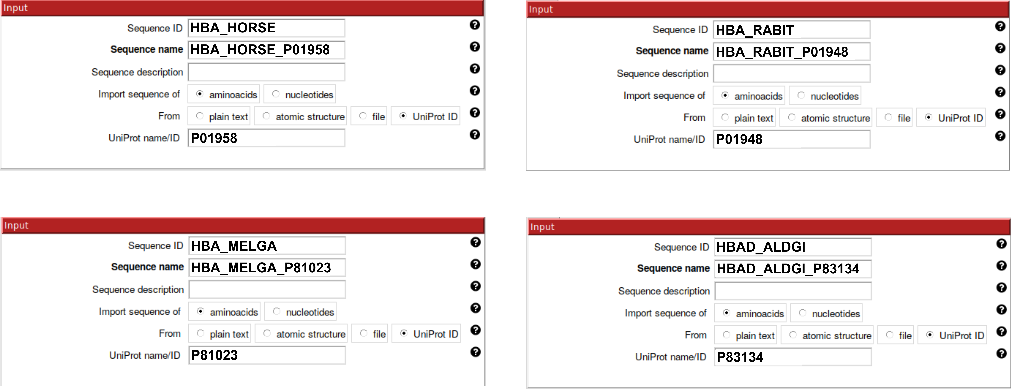
\includegraphics[width=0.95\textwidth]{Images/Fig12}
  \caption{Importing additional sequences to perform the multiple sequence alignment.}
  \label{fig:multialignment_sequences}
  \end{figure}

 \item Access to \modeller in \chimera:\\
 The protocol \scommand{model from template} allows direct opening of the multiple sequence alignment in \chimera and then, access to \modeller via web service. Fill in the protocol form (\ffigure{fig:model_from_template_protocol} (1)), including the \iii{template} \ttt{1PBX} previously imported (2), the particular chain of interest (use the wizard to select it (3)) and the \iii{target} sequence of human \ttt{Hgb} $\alpha$ subunit (4). Since we plan to improve the alignment by including additional sequences to align (5), they will have to be added next (6). Finally, select one of the multiple sequence alignment tools (7). 
 
 \begin{figure}[H]
  \centering 
  \captionsetup{width=.9\linewidth} 
  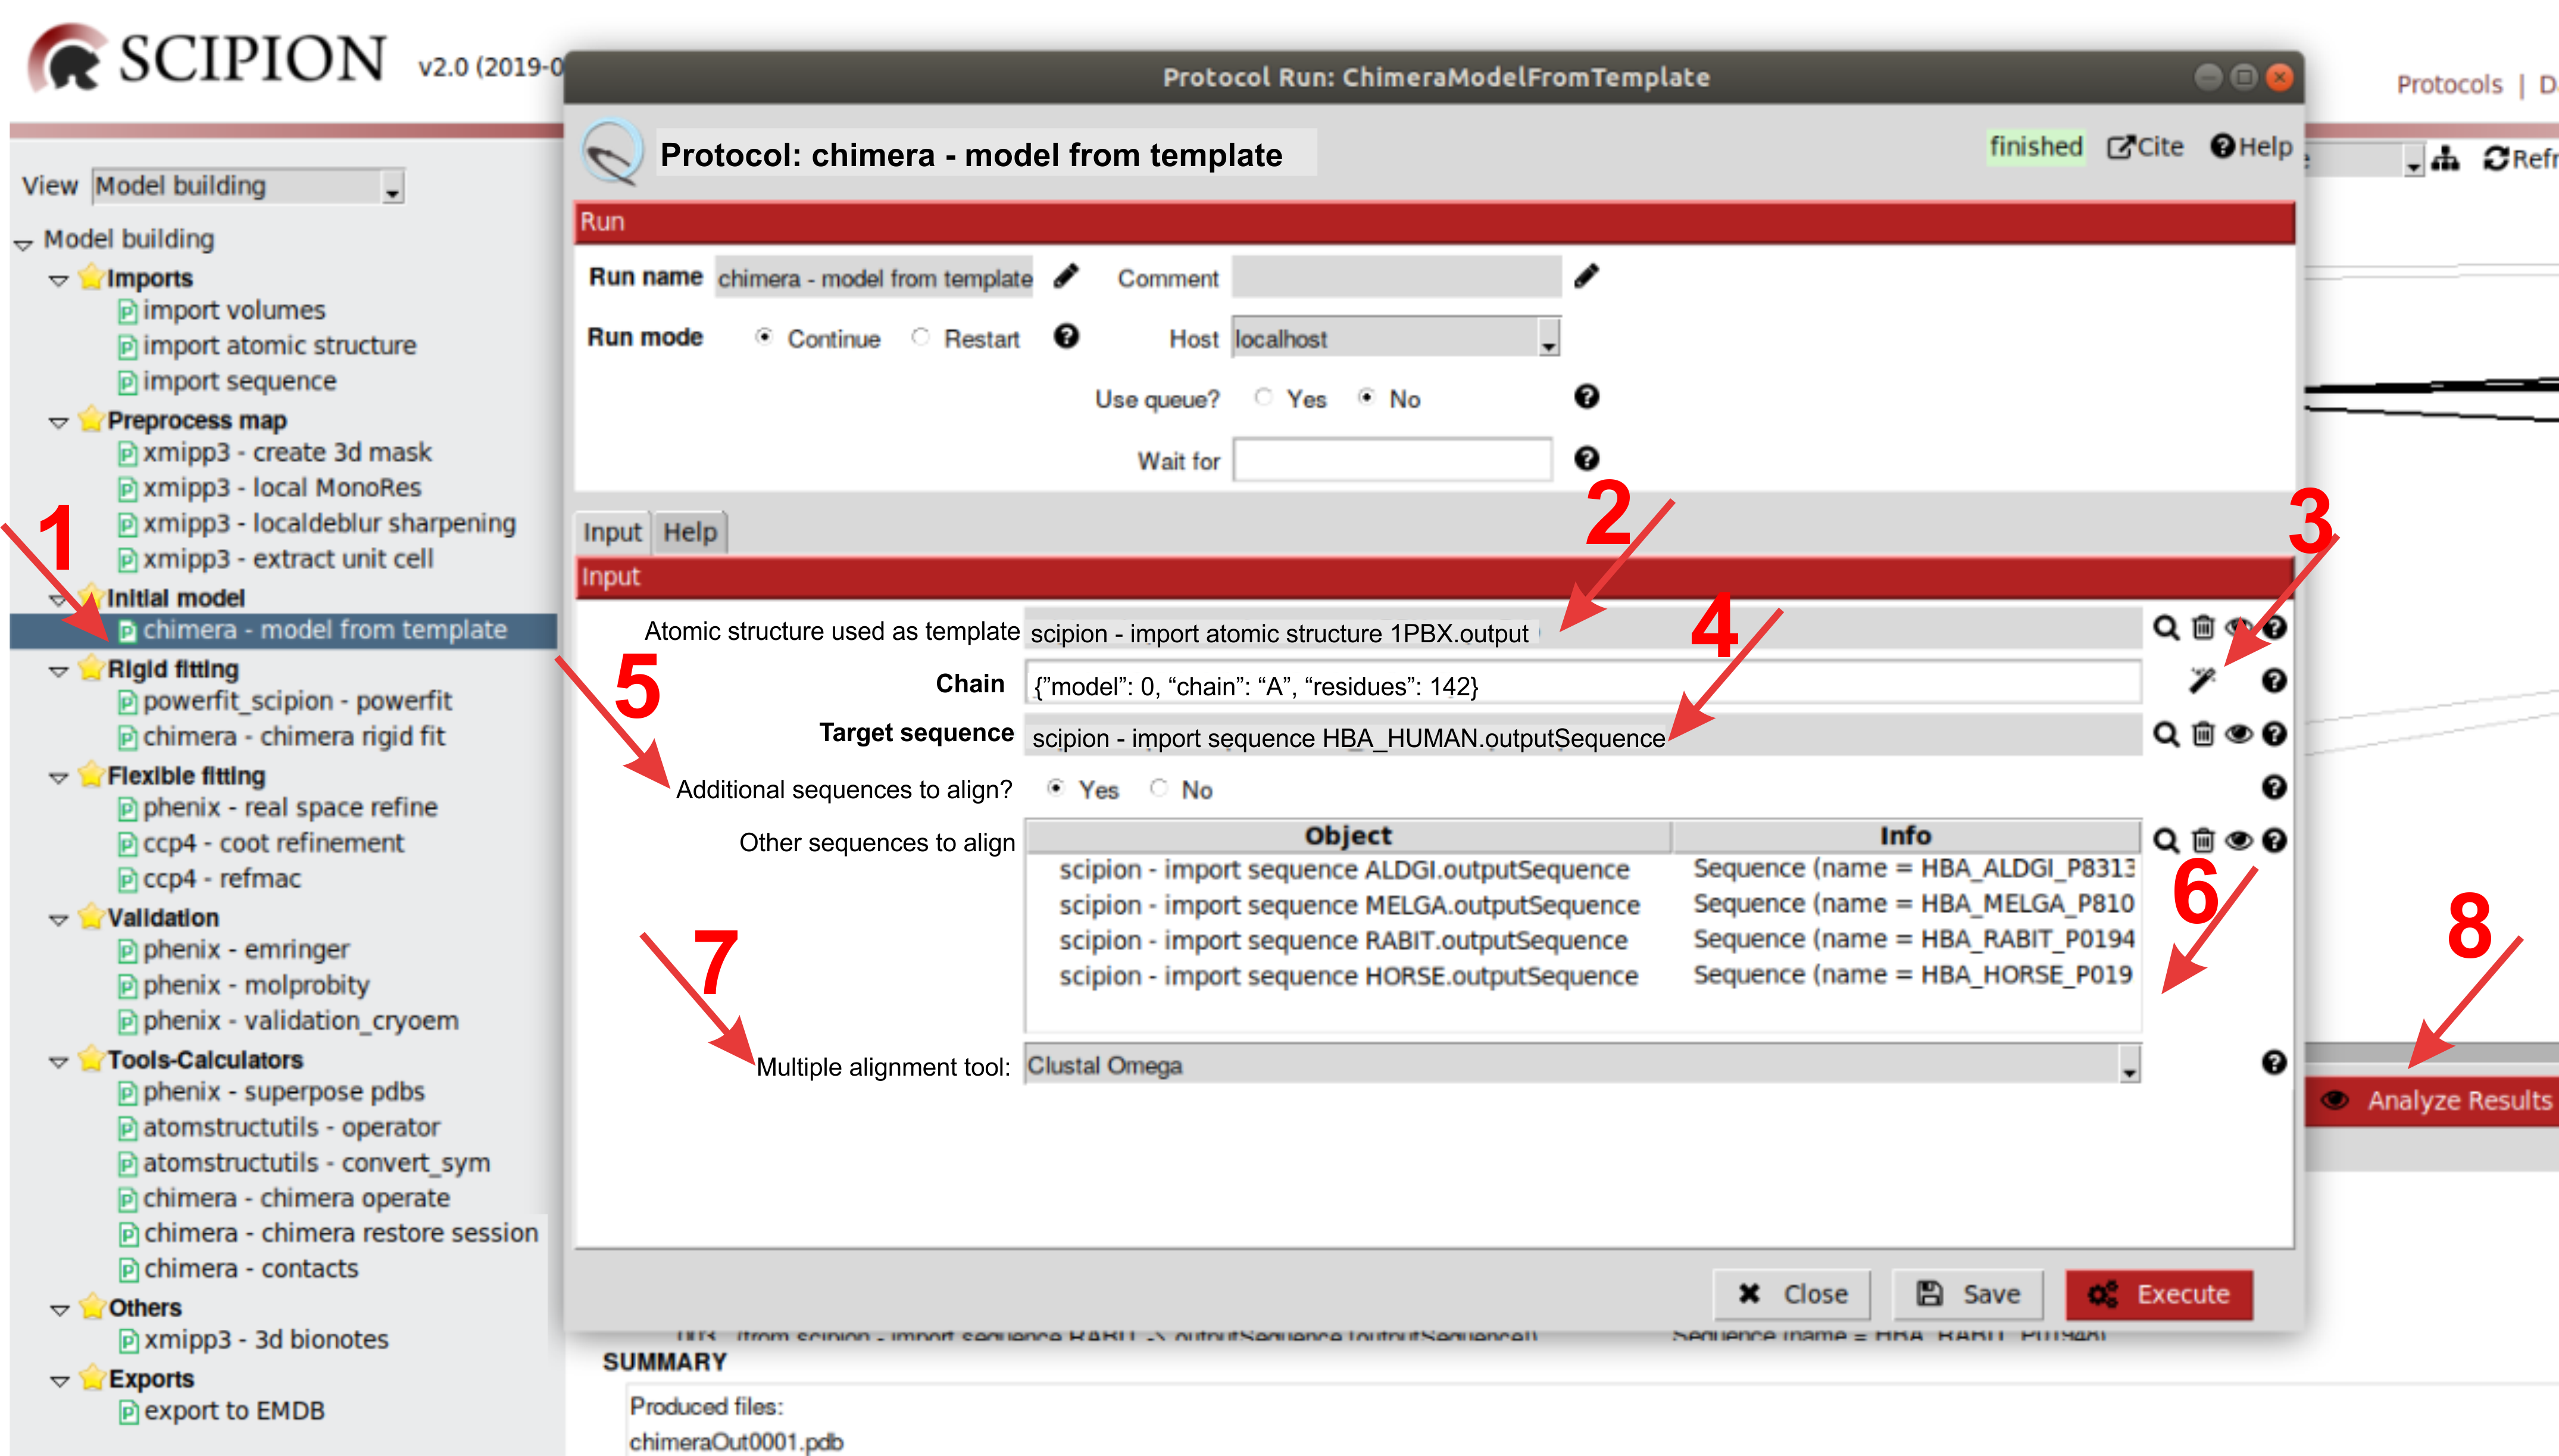
\includegraphics[width=1\textwidth]{Images/Fig13}
  \caption{Importing the multiple sequence alignment in \chimera.}
  \label{fig:model_from_template_protocol}
  \end{figure}
 
 \chimera will be open including this time the multiple sequence alignment together with the \chimera graphics window (\ffigure{fig:chimera_alignment}). The \iii{template} selected chain is shown green-highlighted in both windows. As you may observe in the alignment, \ttt{Hgb} $\alpha$ subunit is a quite conserved macromolecule; there is only one gap in the alignment because \ttt{PRO} (Proline) 47 residue has disappeared throughout the evolutionary process. 
 %Human \ttt{Hgb} $\alpha$ subunit is closer to the protein in mammals (horse, rabbit) than to the protein in unrelated organisms, as we would have anticipated. Corroborate this point by checking the identity percentage \%ID  between human sequence and the other sequences in \ffigure{fig:modeller} (B). 
 
 \begin{figure}[H]
  \centering 
  \captionsetup{width=.7\linewidth} 
  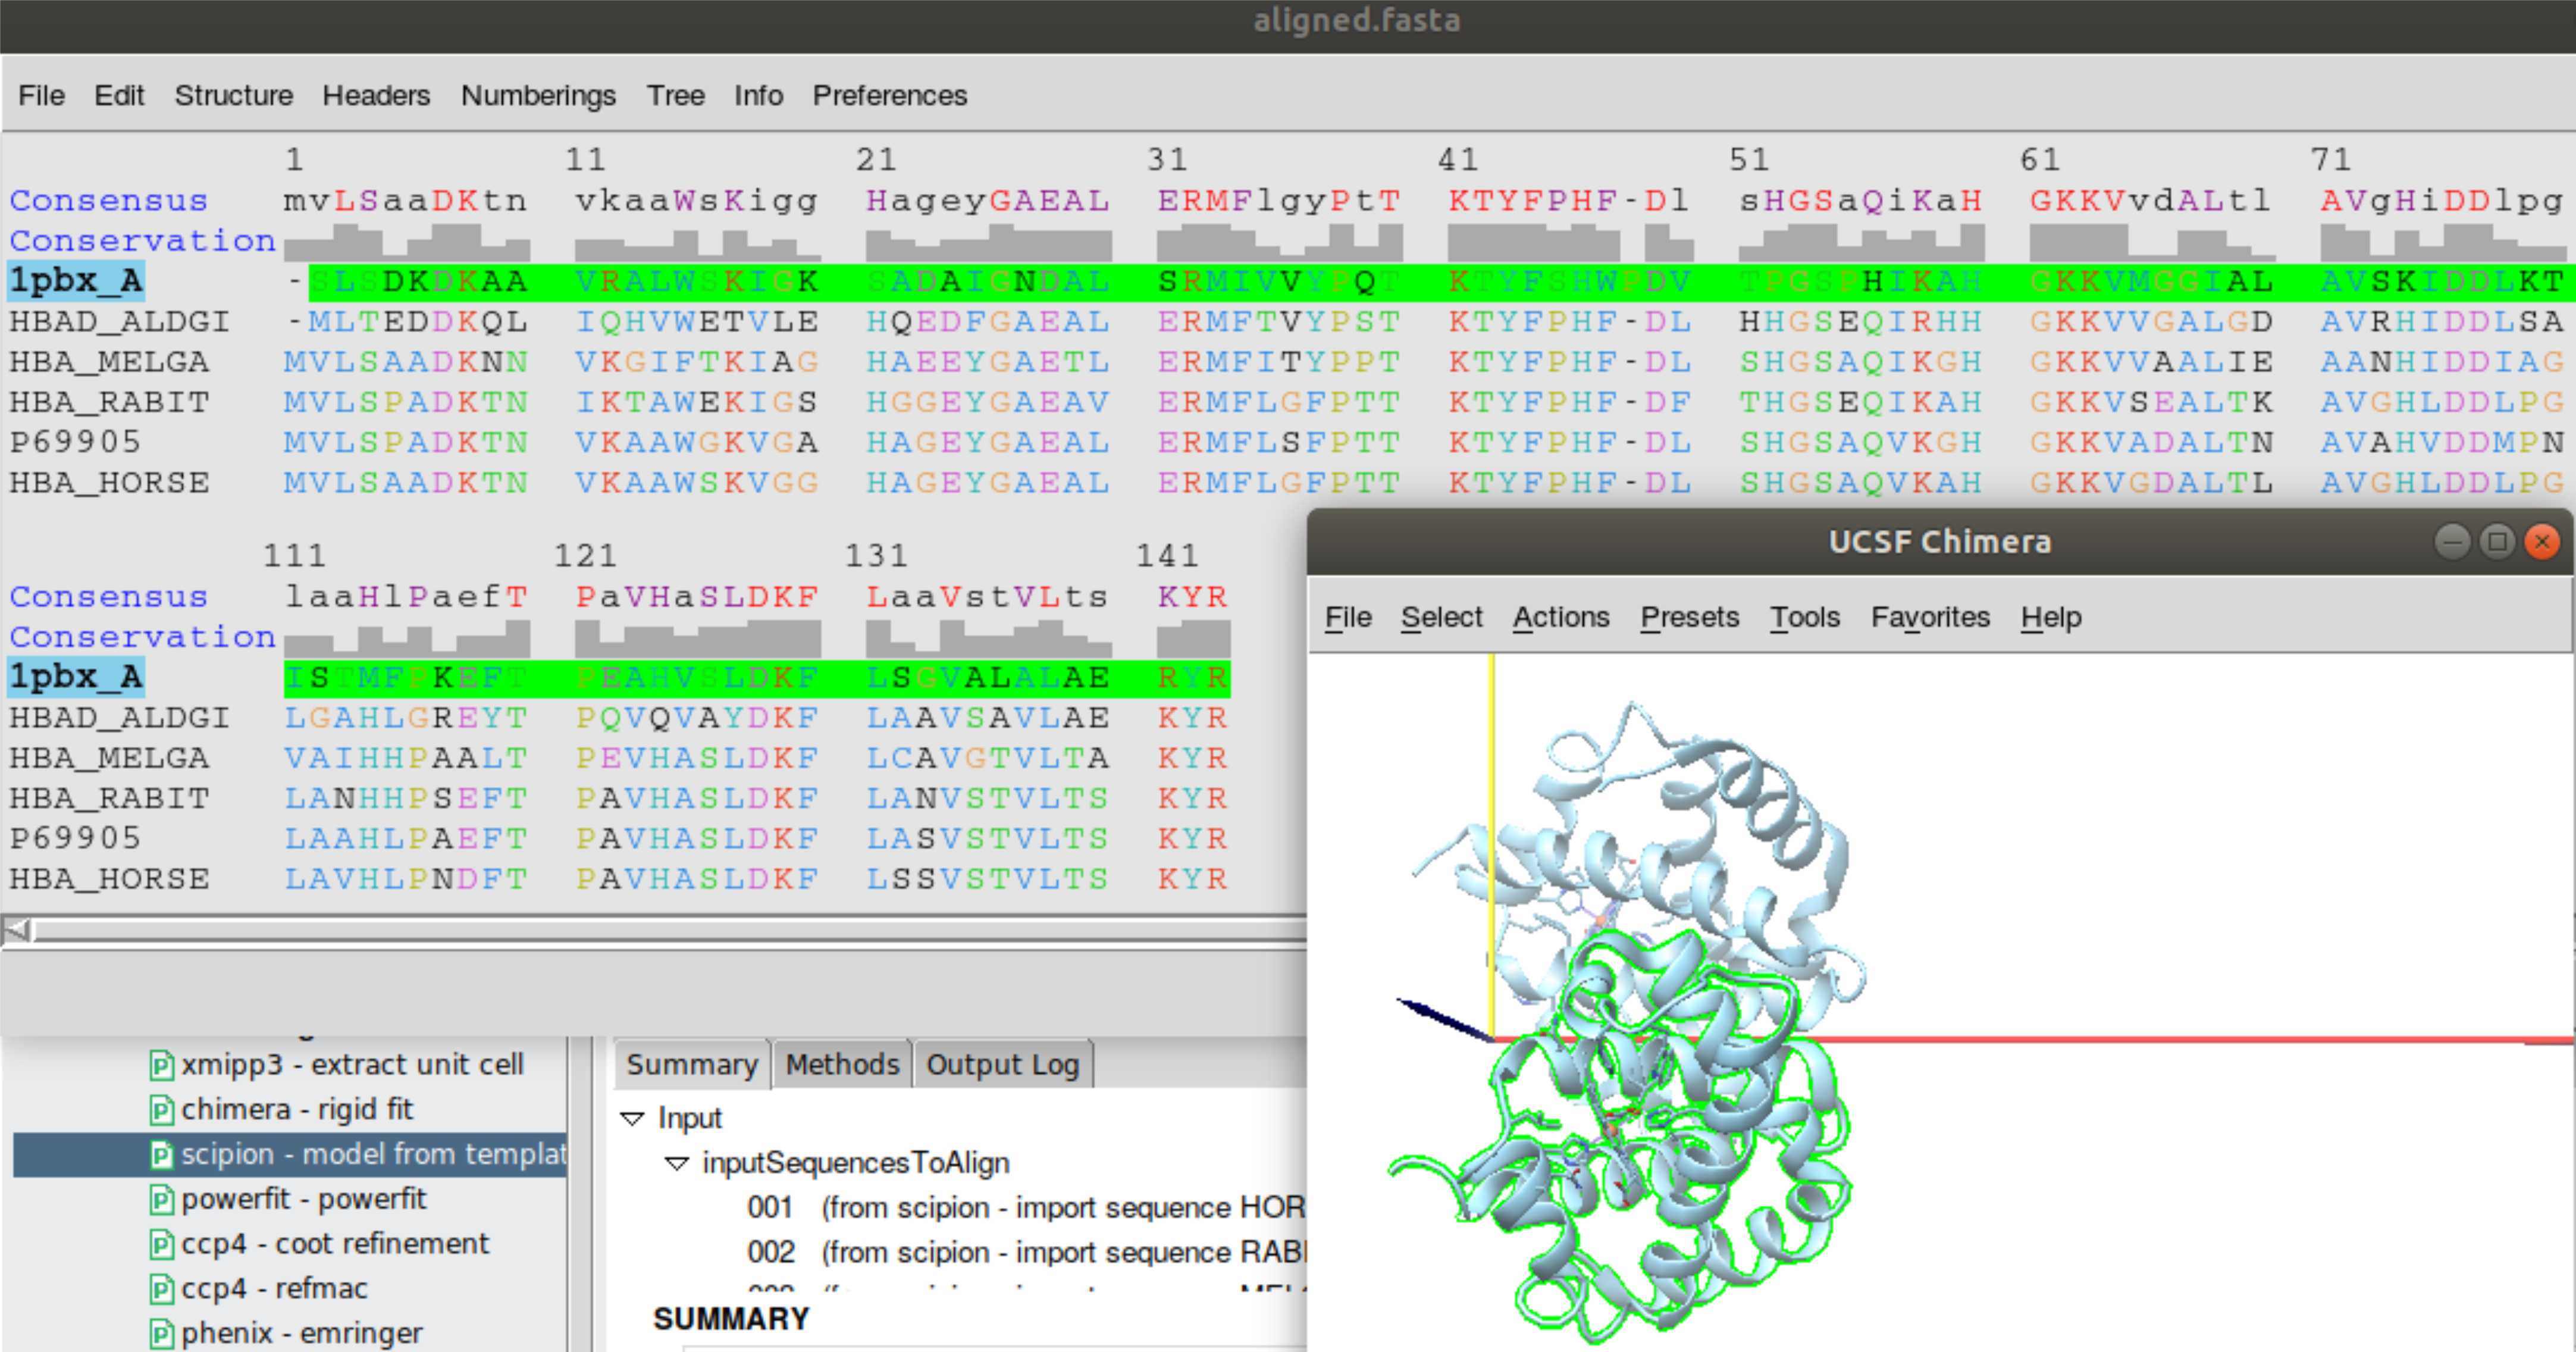
\includegraphics[width=0.80\textwidth]{Images/Fig14}
  \caption{Opening the multiple sequence alignment in \chimera.}
  \label{fig:chimera_alignment}
  \end{figure}
\end{itemize}

%In case you'd like edit the name or the order of the sequences, add,  delete or realign sequences, ..., go to the upper menu of the multiple sequence alignment (\ttt{Edit -> }). In particular, we are going to change the name of the \iii{target} sequence from \ttt{P69905} to \ttt{HBA\_HUMAN} in \ttt{Edit -> Edit Sequence Name...} (\ffigure{fig:modeller} (A)).
To complete the form that will allow us to get any atomic model of the \iii{target} sequence in \modeller web service, we have two possibilities: a) to select \ttt{Tools} (\ffigure{fig:chimera_alignment}, red arrow) \ttt{-> Sequence -> Modeller Comparative}, or b) clicking with the right mouse inside the \ttt{Seqview} box (\ffigure{fig:chimera_alignment}, green arrow) and selecting \ttt{Structure -> Modeller Comparative Modeling...} in the pop up window. A new window of \ttt{Modeller Comparative} will be open (\ffigure{fig:modeller} (A)), that we have to fill in. \ttt{Sequence alignments} (1) should include the \iii{template} sequence. In \ttt{Target sequences} section (2) we should include the \iii{target} sequence that we would like to model, \ttt{HBA\_HUMAN\_P69905} in this particular case. Modeller license key has to be included here (3). The number of output models, 5 by default, can be also specified (4). Since the target sequence that we would like to model should include \ttt{non-water HETATM residues} (\ttt{HEME} group) we are going to select this as \ttt{Advance option} (5). Finally, press \ttt{OK} (6) to start the computation of potential models for your \iii{target} sequence.\\

  \begin{figure}[H]
  \centering 
  \captionsetup{width=.7\linewidth} 
  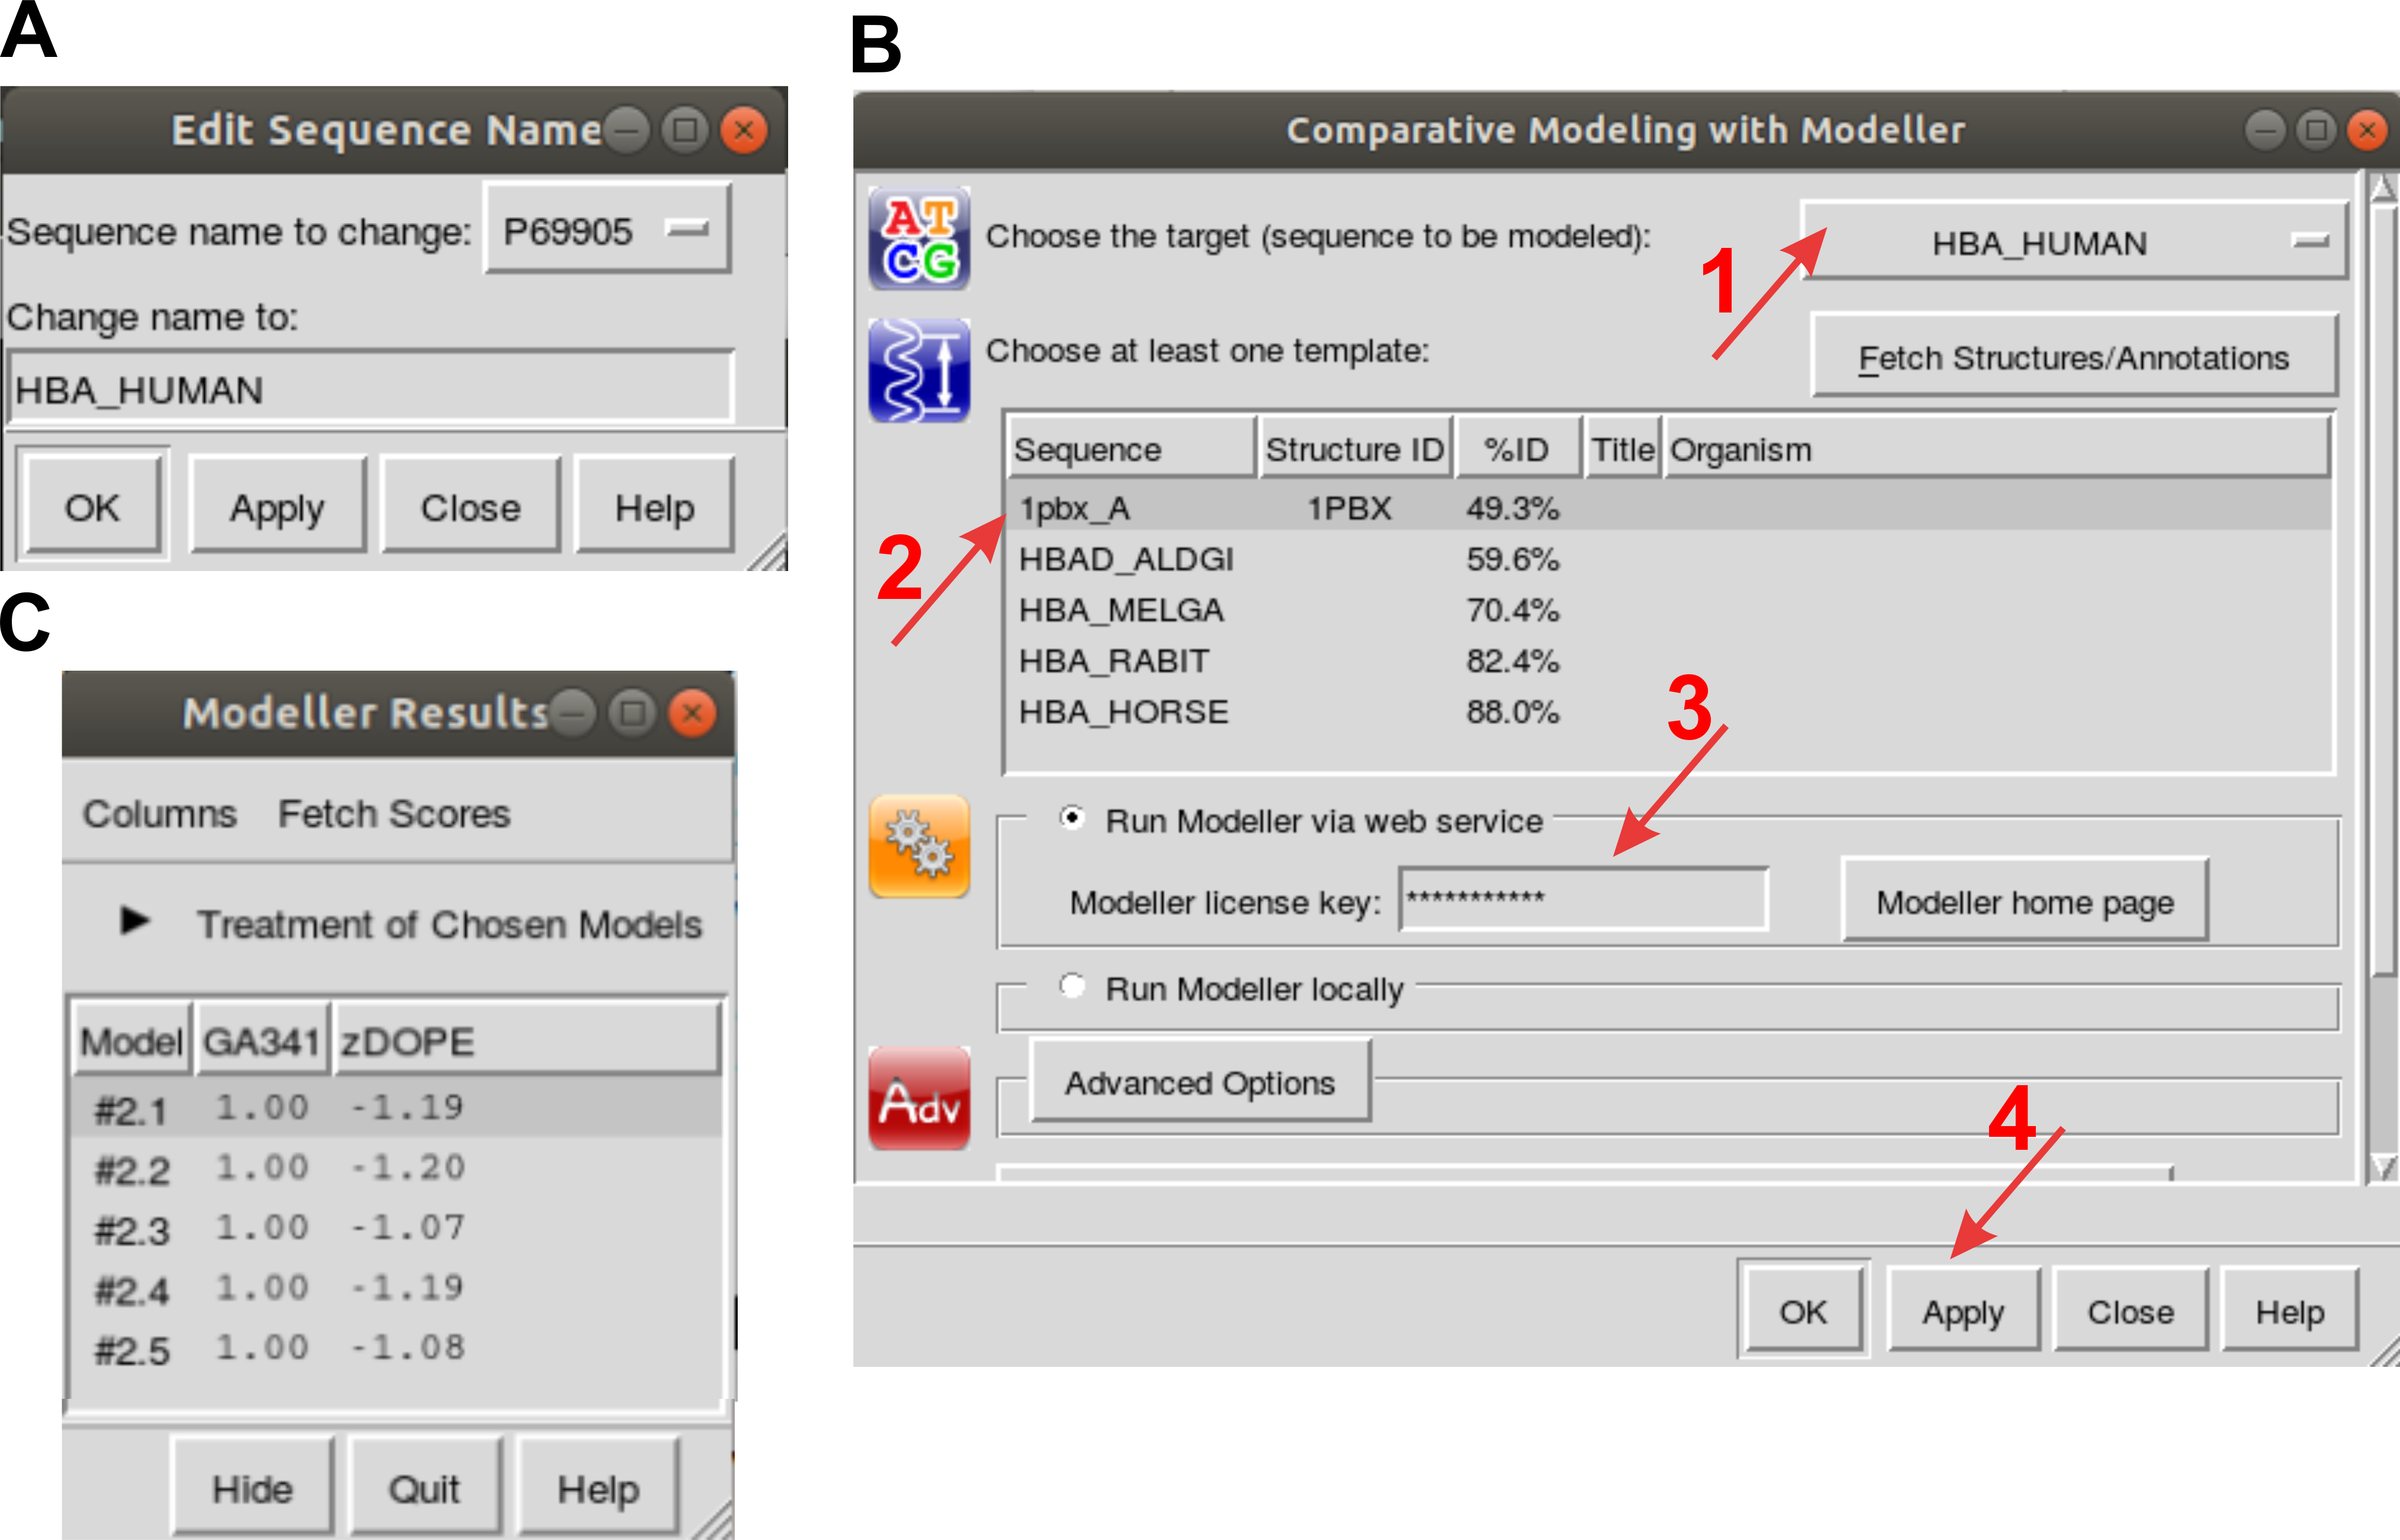
\includegraphics[width=0.7\textwidth]{Images/Fig15}
  \caption{(A) Completing the form to access to homology modeling with \modeller. (B) Resulting \iii{model scores}. (C) \chimera \ttt{Model panel}}
  \label{fig:modeller}
  \end{figure}

In \chimera main graphics window, lower left corner, you may see the status of your job. After a while, five possible atomic structures, from now ahead \iii{models}, are retrieved for the \iii{target} sequence (\ffigure{fig:modeller} (B)) together with their assessment scores. Column \ttt{GA341} of Modeller Results indicates the score derived from statistical potentials (values in \ttt{[0,1]}; \ttt{> 0.7} for reliable \iii{models}). Column \ttt{zDOPE} (normalized Discrete Optimized Protein Energy) score depends on the atomic distance (negative values for the better \iii{models}). You can check every model numbers in \chimera's main menu (\ttt{Tools -> Models} (C)).

For this tutorial we are going to select \iii{model} \ttt{\#3.2}  (\ffigure{fig:modeller} (B), green arrow). Renaming this model is the first step to save it. We can rename the model by typing in the \chimera command line:
 \begin{verbatim}
     rename #3.2 id #4
 \end{verbatim}
The renamed atomic structure will appear in the \ttt{Models} panel (\ffigure{fig:modeller} (C), green arrow). To track this new atomic structure in the \scipion workflow, we can write in the \chimera command line:
\begin{verbatim}
     scipionwrite #4 prefix model_from_modeller_3_2_
 \end{verbatim}
 
In case that the \ttt{Advanced option} \ttt{'Include non-water non-water HETATM residues from template'} was temporally disabled ((\ffigure{fig:modeller} (A, 5)), an alternative option to have the model with the \ttt{HEME} group (residue 144 from the atomic structure #2 chain A) could be:
\begin{verbatim}
     rename #3.2 id #4
     select #4
     select add #2/A:144
     save /tmp/tmp.cif format mmcif models #2,4 selectedOnly true
     open /tmp/tmp.cif
     scipionwrite #5 prefix model_from_modeller_3_2_
 \end{verbatim}


 
 \begin{figure}[H]
  \centering 
  \captionsetup{width=.7\linewidth} 
  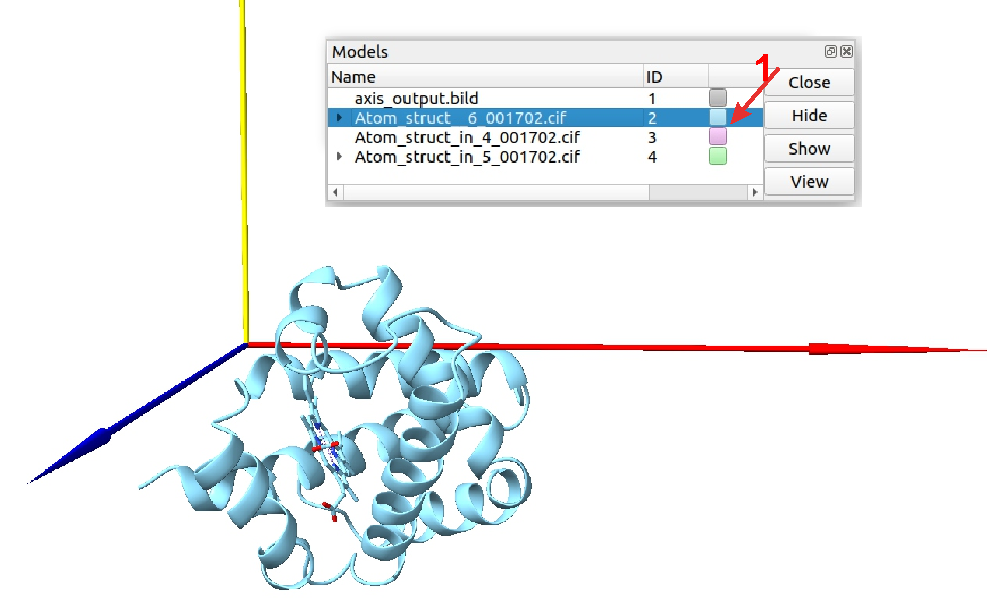
\includegraphics[width=0.80\textwidth]{Images/Fig16}
  \caption{\iii{Model} selection in \chimera. (A) Selected \iii{model} \ttt{\#2.1}. (B) Creation of full final \iii{model} of human \ttt{metHgb} $\alpha$ subunit, including \ttt{HEME} group.}
  \label{fig:chimera_model}
  \end{figure}
 
 After closing \chimera, you can visualize (\ffigure{fig:model_from_template_protocol} (8)) your full predicted \iii{model}. In a similar process, you can also obtain human \ttt{metHgb} $\beta$ subunit. %Remark that in this case, the \ttt{HEME} group will be kept with the next \chimera command line: \\
 %\ttt{delete \#1:.A, 0-147.B, 149-.B}\\ or \\
 %\ttt{delete \#1:.A}\\ \ttt{delete \#1:0-147.B}\\ \ttt{delete \#1:149-.B}\\
 Use this time a direct way of keeping the \ttt{HEME} group in your $model$ of \ttt{metHgb} $\beta$ subunit: Select the advanced option \ttt{Include non-water HETATM residues from template} included in  \ttt{Comparative Modeling with Modeller} window (\ffigure{fig:modeller} (B)).\\
  
If for any reason you decide to go back and check a different \iii{model} from the five \iii{models} initially provided by \modeller, you can do it by using \scommand{chimera restore session} protocol (Appendix \ref{app:chimeraRestoreSession}). This protocol may be used whenever \chimera session had been saved, specifically after using protocols \chimera \ttt{rigid fit}, \chimera \ttt{operate}, and \chimera \ttt{model from template}. In addition to the \chimera command line \ttt{scipionss}, command line \ttt{scipionwrite} also saves \chimera session by default. So, if you want to restore a previous session just open the form (\ffigure{fig:restore_session_protocol}, 1), and include the session that you'd like to restore (2).

 \begin{figure}[H]
  \centering 
  \captionsetup{width=.7\linewidth} 
  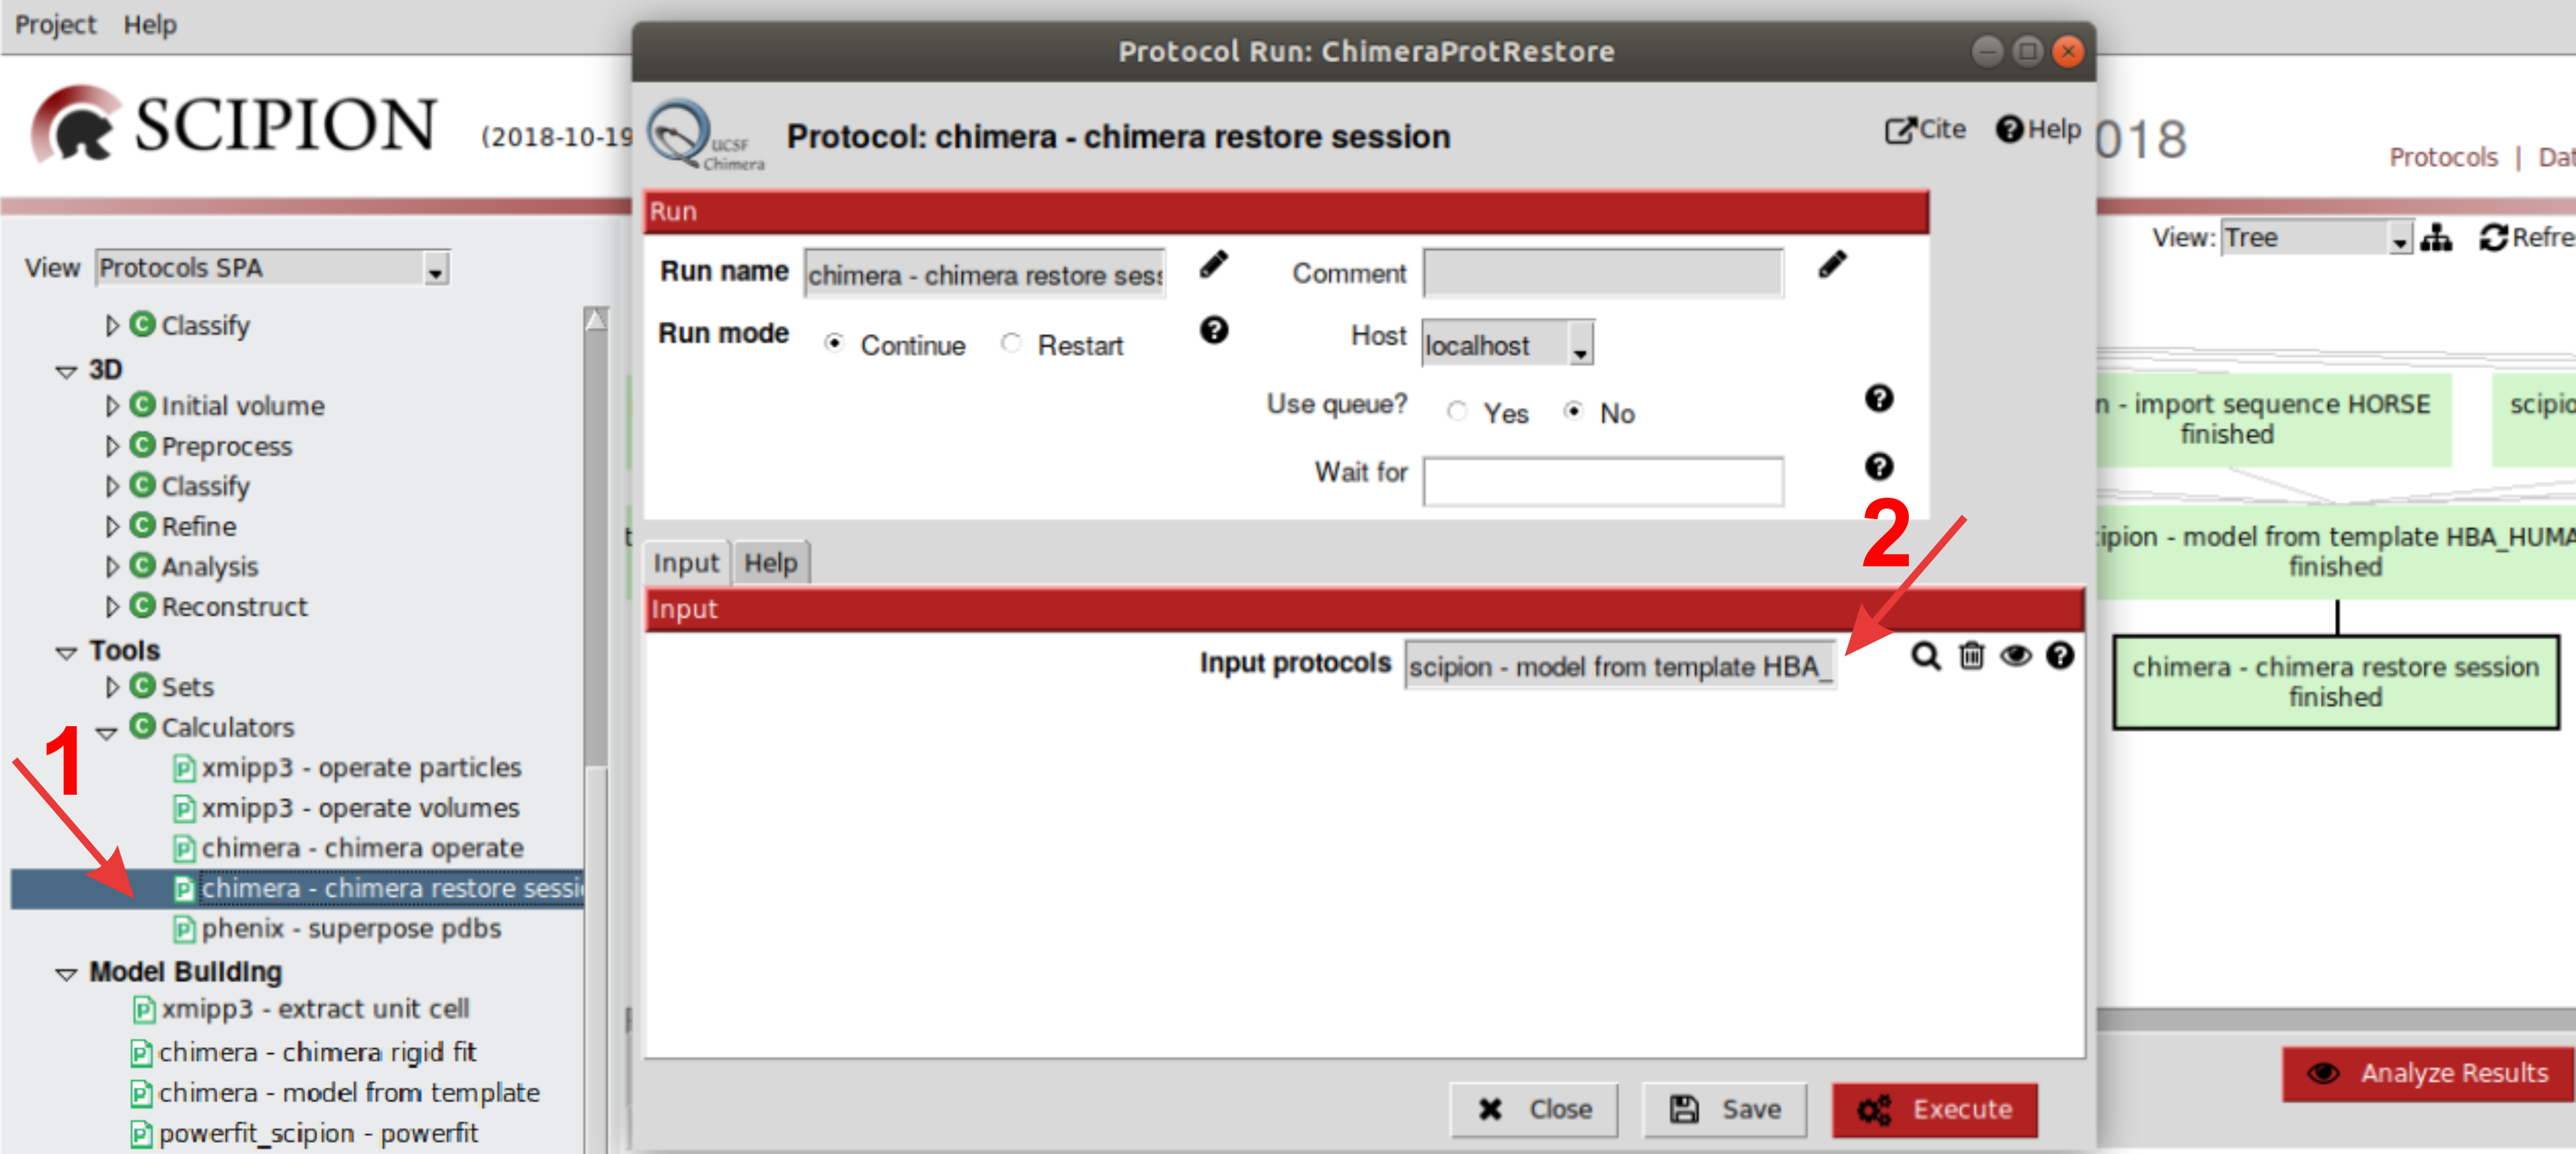
\includegraphics[width=0.90\textwidth]{Images/Fig17}
  \caption{Restoring session in \chimera.}
  \label{fig:restore_session_protocol}
  \end{figure}
